\section{Introduction}
ALL TEXT SURROUNDED BY [] LIKE \cite{lab3 Manual} SHOULD BE CLICKABLE AND LEAD
EITHER TO WEBPAGE OR PLACE IN THIS DOCUMENT \\
The goal of the laboratory was to create three scenarios using config file and
then investigate how those scenarios played out. \\
Scenario 1: 2 Processes \\
Scenario 2: 5 Processes \\
Scenario 3: 10 Processes \\
We had to get to know how the schedulers work, how they switch. \cite{lab3
Manual} 
\paragraph{First come first serve}
We used First come first serve algorithm $\rightarrow$ This algorithm simply executes the process which
arrived first. The process that requests CPU as a first process gets the CPU
first. It is easy to implement and understand. We just use Queue data structure
and we pick processes from the head of the queue and new procesess are added at
the tail of the queue. \cite{First come first serve}
\begin{figure}[H]
	\caption{First come first serve example graphic from
		\href{https://www.geeksforgeeks.org/program-for-fcfs-cpu-scheduling-set-1/}{[Geeks for
	Geeks]}}
	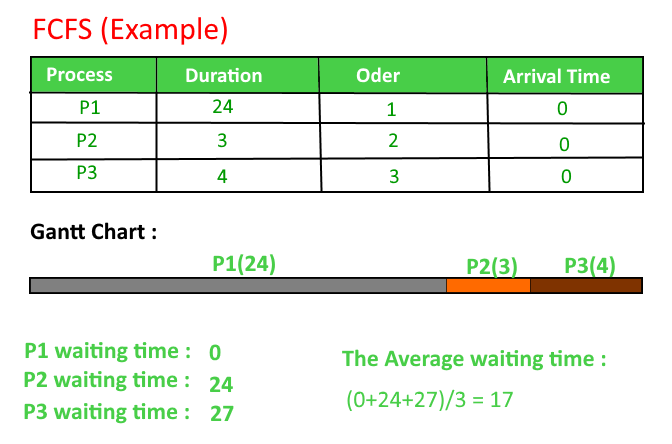
\includegraphics[width=\textwidth]{FCFS}
\end{figure}
\paragraph{Other algorithms} \cite{Other scheduling algorithms}
\begin{enumerate}
	\item Shortest-Job-Next - Executes first processes that will take least
		time to finish
	\item Priority Scheduling - Each process gets assigned a prority and we
		execute them from the process with highest priority to the
		process with lowest prority
	\item Round Robin Scheduling - We give each process a constant time to
		execute, after this time expires regardless whether process
		finished or not we go to another process untill all of them are
		finished
\end{enumerate}
